\documentclass[wcp]{jmlr}
\usepackage{booktabs}
\usepackage{lineno}
\providecommand{\doi}[1]{\href{https://doi.org/#1}{doi:~\nolinkurl{#1}}}
\hypersetup{pageanchor=false}
\pagenumbering{gobble}
\makeatletter
\let\Ginclude@graphics\@org@Ginclude@graphics
\makeatother
\jmlryear{2026}
\jmlrworkshop{ACML 2026}
\title[Active Learning for Protein--Lipid Affinity]{Discovery, Prediction, and Explanation in Active Learning for Protein--Lipid Binding Affinity}
\author{}
\editors{Andy Song, Bo Han and Sarah Erfani}
\begin{document}
\makeatletter\let\@jmlrpages\@empty\makeatother
\maketitle
\begin{abstract}
Active learning for molecular affinity can prioritize strong binders without
necessarily improving prediction over the full candidate distribution. We
examine this distinction in a retrospective protein--lipid benchmark assembled
from published measurements. Two pooled BioDolphin endpoints contain 864 and
549 deduplicated protein--lipid pairs, while four small target panels contain
11--16 pairs each. We evaluate five lipid representations, including three
frozen molecular transformers, five Gaussian-process kernels and 13 query
policies, yielding 5,850 campaigns across three seeds. Uncertainty-only
acquisition gives the lowest descriptive mean MAE on pooled dissociation
and inhibition affinities (0.641 and 0.429 pK), whereas a Thompson
configuration on dissociation affinities recovers 96.7\% of the pool's
top-decile pairs with MAE 0.705. Prediction and discovery rankings therefore
disagree. We complement final-model grouped SHAP with 14,754 ungrouped ECFP
explanations across 396 cycle snapshots, including affinity-prioritized
fragment visualization and protocol stability analysis. Exact affine-model
attributions agree with independent KernelExplainer checks to below
$10^{-10}$ pK. These checks establish computational fidelity, not mechanistic
validity. Random-pair splits, heterogeneous assays, small target panels, and
post-hoc configuration selection limit generalization claims. The study
provides an auditable domain adaptation and exposes the distinction between
acquisition success, predictive quality, and chemical interpretation. A
companion dashboard exposes the complete grid and local measured-data campaigns.
\end{abstract}
\begin{keywords}
active learning; protein--lipid affinity; Gaussian processes; Thompson sampling; SHAP; retrospective evaluation
\end{keywords}

\section{Introduction}
Protein--lipid interactions present a useful setting for evaluating molecular
active learning: experiments are limited, the candidate space is chemically
heterogeneous, and collecting strong binders is not the same objective as
predicting every affinity accurately. A policy that repeatedly selects
high-scoring pairs may enrich its measured set while neglecting regions of
the distribution needed for accurate global prediction. This distinction
should be made explicit when evaluating an acquisition policy.

Published protein--lipid resources enable retrospective evaluation, but their
size can be misleading if structural contacts are treated as independent
quantitative measurements. BioDolphin supplies a broad interaction resource
\citep{yang2024}; only its curated affinity-bearing subset is used here.
Separate TRAAK measurements provide much smaller, target-specific panels
\citep{schrecke2021}. These sources offer complementary evaluation regimes,
not six independent large-scale biological studies.

We adapt the ligand-affinity framework of \citet{srivastava2026} to pairwise
protein--lipid prediction. This is an empirical transfer and audit rather
than a new acquisition algorithm. Our contributions are: (i) a matched
representation--kernel--policy grid on measured protein--lipid affinities;
(ii) separate evaluation of held-out prediction and acquisition-pool
enrichment; (iii) cycle-resolved, chemically annotated explanations with
explicit numerical and interpretive checks; and (iv) an interactive results
portal that separates complete benchmark coverage from selected SHAP analyses.
Negative findings on tiny panels
and disagreement between predictive and discovery objectives are retained,
rather than obscured by reporting only the most favorable scores.

\section{Related Work and Scope}
Gaussian-process molecular active learning combines a surrogate mean with
uncertainty-aware querying. The reference framework compares molecular
encodings, covariance functions and scheduled exploration/exploitation
\citep{srivastava2026}. We retain its grid structure and add joint-posterior
Thompson sampling \citep{russo2018}: a correlated function realization is drawn over the
remaining pool, and the highest sampled values form the next batch. The
method does not replace that joint draw by independent uncertainty noise.

SHAP provides additive attributions relative to a specified background game
\citep{lundberg2017}. In molecular applications, assigning importance to a
fingerprint bit does not uniquely identify a chemical fragment because
hash collisions and repeated environments are possible. Furthermore,
feature replacement can leave the manifold of valid molecules. We separate
numerical attribution checks, structural annotations, and biological claims.
No prospective experiment, protein-contact analysis or validated binding
pose is provided. Neither learned protein embeddings nor a newly trained
deep kernel is evaluated. ChemBERTa-MTR, ChemBERTa-MLM and MoLFormer
are frozen lipid encoders; their use is not a claim of a novel transformer.

\section{Data and Evaluation Design}
\subsection{Measured datasets}
Table~\ref{tab:data} lists the benchmark subsets. Positive quantitative
affinities are converted to $\mathrm{p}K=-\log_{10}(K/\mathrm{M})$, so higher
values indicate stronger affinity. The pooled $K_d$ and $K_i$ endpoints
remain separate. Deduplication is by protein sequence and lipid SMILES;
the curated median is an aggregation of source records, not a newly measured
affinity. Censored annotations are excluded. BioDolphin's broad lipid
definition is not restricted to membrane phospholipids. Its imported assay
annotations may originate in other affinity resources; this benchmark does
not claim that all measurements were generated by BioDolphin itself.

TRAAK panels use the mean first sequential binding constant, $K_{d1}$,
from the published triplicates. Replicates and subsequent binding events
are not counted as additional training pairs. Two transthyretin (TTR)
sequence-defined subsets are drawn from BioDolphin and overlap its pooled
$K_d$ panel. The two publications are the independent data sources;
endpoints, constructs and subsets are not independent replications.

\begin{table}[t]
\centering
\caption{Curated benchmark subsets and acquisition budgets. TTR-A and TTR-B
denote the sequence-defined subsets with identifiers 889201f64e9f and
e1eca46439c9, respectively. Small panels are exploratory.}
\label{tab:data}
\begin{tabular}{lrrrr}
\toprule
Panel & Pairs & Test pairs & Initial labels & Final labels\\
\midrule
BioDolphin $K_d$ &864&173&60&360\\
BioDolphin $K_i$ &549&110&60&360\\
TRAAK-a $K_{d1}$ &16&3&2&8\\
TRAAK-b $K_{d1}$ &16&3&2&8\\
TTR-A $K_d$ &11&2&2&8\\
TTR-B $K_d$ &11&2&2&8\\
\bottomrule
\end{tabular}
\end{table}

\subsection{Splits, budgets, and metrics}
Seeds 7, 19 and 42 define matched random-pair partitions. Approximately
20\% of rows are frozen as test data; test labels never guide querying or
model fitting. Each pooled campaign begins with 60 labels and acquires
ten batches of 30. This measures 360 of 691 eligible $K_d$ pairs and 360
of 439 eligible $K_i$ pairs. The latter budget covers about 82\% of its
pool, making high final recall less demanding than early discovery.
Small panels start with two labels and distribute six further labels
over ten phase slots as $(0,1,0,1,1,0,1,0,1,1)$. Zero-budget phases do not
refit the model. Their schedules preserve phase positions but do not
reproduce the large-panel measurement budget.

We report held-out MAE in pK units and $R^2$, separately from top-decile
recall in the acquisition pool. The hit set contains the top
$\lceil0.1N_{\mathrm{pool}}\rceil$ affinities, including ties at the threshold;
initial labels count toward recall. Recall AUC is the trapezoidal area
under recall versus number of labels, divided by the acquired-label range.
It captures discovery timing rather than only the endpoint. The experiments
also record top-2\% and top-5\% recall, RMSE, simple regret and 90\%
predictive-interval coverage.

Configurations share test partitions and initial labels within a seed.
Consequently, configurations are not independent replicates. Reported
means and standard deviations refer to the three seeds. Selecting a
configuration by its observed test MAE or recall AUC makes it a descriptive
winner, not an unbiased estimate of a validated model-selection procedure.
No significance claim is made from three seeds or overlapping panels.

\section{Surrogates and Acquisition}
\subsection{Representations and pairwise covariance}
Lipid inputs are radius-4, 4096-bit Morgan fingerprints (ECFP; \citealp{rogers2010}), RDKit's
167-output-bit MACCS representation, fixed 384-dimensional
ChemBERTa MTR and MLM CLS embeddings (77M checkpoints)
\citep{chemberta}, and 768-dimensional masked-mean MoLFormer-XL embeddings
\citep{ross2022}. Radius four follows the reference
implementation and corresponds to diameter-eight terminology; we do not
silently relabel it as radius-two ECFP. All 549 distinct lipid strings are
encoded without truncation: maxima are 156 ChemBERTa and 154 MoLFormer tokens.
The latter checkpoint is pretrained on 10\% of both ZINC and PubChem;
canonical non-isomeric SMILES match its stereochemistry-removing preprocessing.
This loss of stereochemical information is a representation limitation.
The encoders are not affinity-fine-tuned. Revisions and feature hashes are
pinned; all pretrained base-model tensors load strictly. Protein inputs contain 20 amino-acid composition values,
four composition groups, log sequence length and a charge descriptor.

For a pair $z=(p,l)$ we use
\begin{equation}
k(z,z')=s\,k_L(l,l')\,k_P(p,p'),
\end{equation}
where $k_L$ is Tanimoto, linear, RBF, rational quadratic, or Mat\'ern-$3/2$.
The protein factor is Mat\'ern-$3/2$ and becomes one on a constant-protein
panel. Protein standardization and distance scaling use initial inputs
only and remain fixed through the campaign. The dot-product Tanimoto
extension is also evaluated on dense transformer vectors; it is not a binary
chemical-substructure interpretation of those coordinates.

An exact GP \citep{rasmussen2006} learns a constant mean, signal variance
and noise variance. Applicable length scales and the rational-quadratic
shape are also learned by marginal likelihood optimization.
Target normalization uses acquired labels only.
Optimization uses analytic-gradient L-BFGS-B, warm starts and at most 60
iterations per fit. This differs from the reference authors' Adam routine;
the protein covariance factor is also a domain adaptation. Posterior
means and variances, hyperparameters, optimization status and row indices
are saved at every fitted round.

\subsection{Query policies}
Write $E$ for ranking by observation predictive standard deviation,
$X$ for ranking by predicted mean, and $B$ for ranking by
$0.5\mu+0.5\sigma$. The schedules are balanced ($B^{10}$), alternate
($(EX)^5$), sandwich ($E^2X^6E^2$), explore-heavy ($E^7X^3$),
exploit-heavy ($X^7E^3$), and gradual ($E^3B^4X^3$), together with
uniform random selection. Thompson sampling draws
\begin{equation}
\widetilde{\boldsymbol f}\sim
\mathcal N(\boldsymbol\mu_{\mathcal U},\boldsymbol\Sigma_{\mathcal U})
\end{equation}
over the unqueried pool $\mathcal U$, using latent rather than observation
covariance, and selects the top batch. A small adaptive Cholesky jitter
stabilizes the joint draw.

The expanded design adds pure exploitation ($X^{10}$), pure uncertainty
($E^{10}$), expected improvement (EI), probability of improvement (PI),
and a Thompson--diversity heuristic. For acquired-label incumbent $y^*$,
$d=\mu-y^*-\xi$, $z=d/\sigma_f$, and $\xi=0.01$ pK, EI is
$d\Phi(z)+\sigma_f\varphi(z)$ and PI is $\Phi(z)$; $\sigma_f$ is latent
posterior SD and zero-variance limits are handled explicitly. Batches select
the largest marginal scores, not joint qEI or noise-integrated EI.
The diversity heuristic standardizes one joint Thompson draw and greedily
adds $0.25[1-\exp(-\min_{j\in S}d_L(i,j)^2/2)]$ to each remaining score,
where $S$ is the within-batch selected set; the first selection has zero bonus.
The distance is initial-input-scaled lipid distance. Constants were fixed
before the expanded runs, not tuned on held-out outcomes. This is a heuristic,
not a new acquisition algorithm or a state-of-the-art claim.

The full design comprises $6\times5\times5\times13\times3=5850$ campaigns,
or 1,950 three-seed configurations. It reuses 2,160 hash-verified original
campaigns and adds 3,690 runs, preserving their splits, budgets and GP engine.
All supported combinations are evaluated; this finite suite is not exhaustive
of the acquisition-function or kernel literature.

\begin{figure}[t]
\centering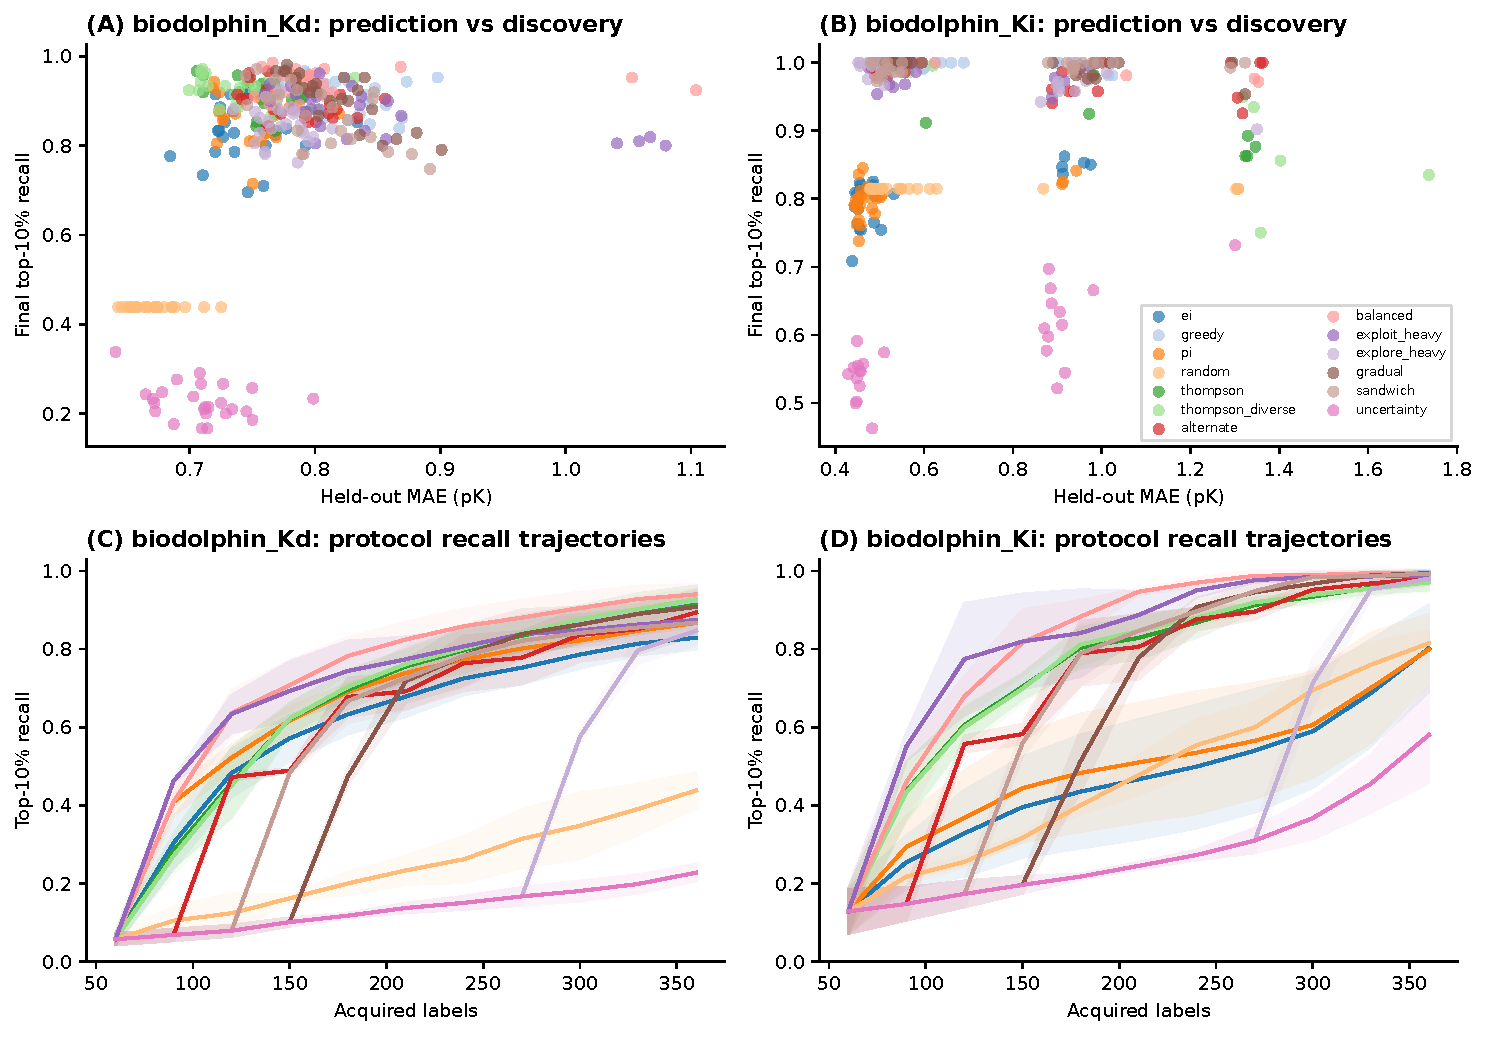
\includegraphics[width=\linewidth]{figures/fig1_performance.pdf}
\caption{Four-panel performance overview. (A,B) Each point is a
three-seed configuration mean, showing that low held-out MAE and high
acquisition recall are different objectives. (C,D) Within each seed,
recall is averaged over the 25 representation--kernel configurations;
lines and shading then show the three-seed mean and standard deviation.
Shading is descriptive variability, not a confidence interval.}
\label{fig:performance}
\end{figure}

\section{Explainability Protocol}
\subsection{Final-model grouped analysis}
For each panel, the original 2,160-run grid's descriptive prediction winner,
discovery winner and lowest-MAE Thompson configuration were explained across
three seeds: 54 saved final models. This explanation cohort is retained,
not reselected using the expanded grid. No SHAP coverage is claimed for all
5,850 runs or for the new MLM/MoLFormer models. Up to eight test pairs are explained using up to
eight acquired-training background pairs. The exact two-player game
separates protein and lipid contributions. A finer permutation-SHAP game
uses 20 training-input-variance-selected fingerprint bits, a joint
remainder-bit group and a joint protein group. ChemBERTa uses 12 embedding
blocks instead. Two independent runs of eight antithetic permutations
provide a sampling-sensitivity diagnostic, not an attribution confidence
interval. Fine-group values and two-player values are different games and
are not added together. Embedding blocks are not named chemical motifs.

\subsection{Cycle-resolved individual-bit explanations}
To follow the temporal chemical analysis of \citet{srivastava2026}, we
compare matched ECFP--linear explore-heavy and exploit-heavy campaigns
on all six panels and all three seeds. We explain the initial model and
ten subsequent cycle snapshots: 36 campaigns and 396 snapshots. Each
cycle draws up to 100 unqueried pairs, excluding frozen test rows, and
up to 50 acquired-training lipids as background. Small panels use all
available observations. All 4096 bits receive individual attributions
before the top ten are selected by mean absolute SHAP.

For pooled data, the query protein is fixed while background lipids are
substituted. The linear lipid kernel then yields an affine posterior
mean $f_p(x)=a+\boldsymbol w(p)^\top x$. For the empirical background
mean $\bar x$, the exact marginal-game Shapley values are
\begin{equation}
\phi_j(x;p)=w_j(p)(x_j-\bar x_j),\qquad
\phi_0(p)=a+\boldsymbol w(p)^\top\bar x.
\label{eq:shap}
\end{equation}
This follows because replacing any subset of coordinates changes the
affine prediction by the sum of their separate effects; every ordering
therefore gives the same marginal contribution. The formula explains
lipid variation conditional on the query protein, not protein main effects.
It cannot be applied to the non-linear lipid kernels.

Equation~\ref{eq:shap} avoids a sampled Kernel SHAP computation for every
pair. One final-cycle pair per campaign is independently checked with
\texttt{KernelExplainer}, using $2M+128$ coalition samples for $M$ varying
coordinates and no L1 feature selection. Replacing the background by its
mean preserves every coalition value exactly for the affine predictor.
This is a disclosed computational shortcut, not a claim to reproduce
the reference implementation's unspecified regularization settings.

\subsection{Fragments and stability}
At each cycle, importance is $N^{-1}\sum_i|\phi_j(x_i;p_i)|$.
Evolution plots follow final top-ranked bits across all cycles, while
per-cycle top-ten lists are also saved. For a selected bit, measured
bit-containing pairs are sorted by descending affinity and an RDKit
environment from the highest-affinity molecule is highlighted. All
environments for that bit in the representative molecule are retained.
We rank fragments by pair prevalence multiplied by mean absolute SHAP;
the algebra of this combined score is an explicit implementation choice.

Affinity distributions for present and absent bits use all measured rows
retrospectively, including held-out rows. These labels do not enter
SHAP, top-bit selection, querying or fitting, but they do enter the
post-hoc fragment display and cannot serve as independent validation.
Protocol and consecutive-cycle stability are measured using top-ten
Jaccard overlap and Spearman correlation over bits active in either
importance vector. Changing the sampled background or unqueried population
can change importance even with an unchanged GP.

\begin{figure}[t]
\centering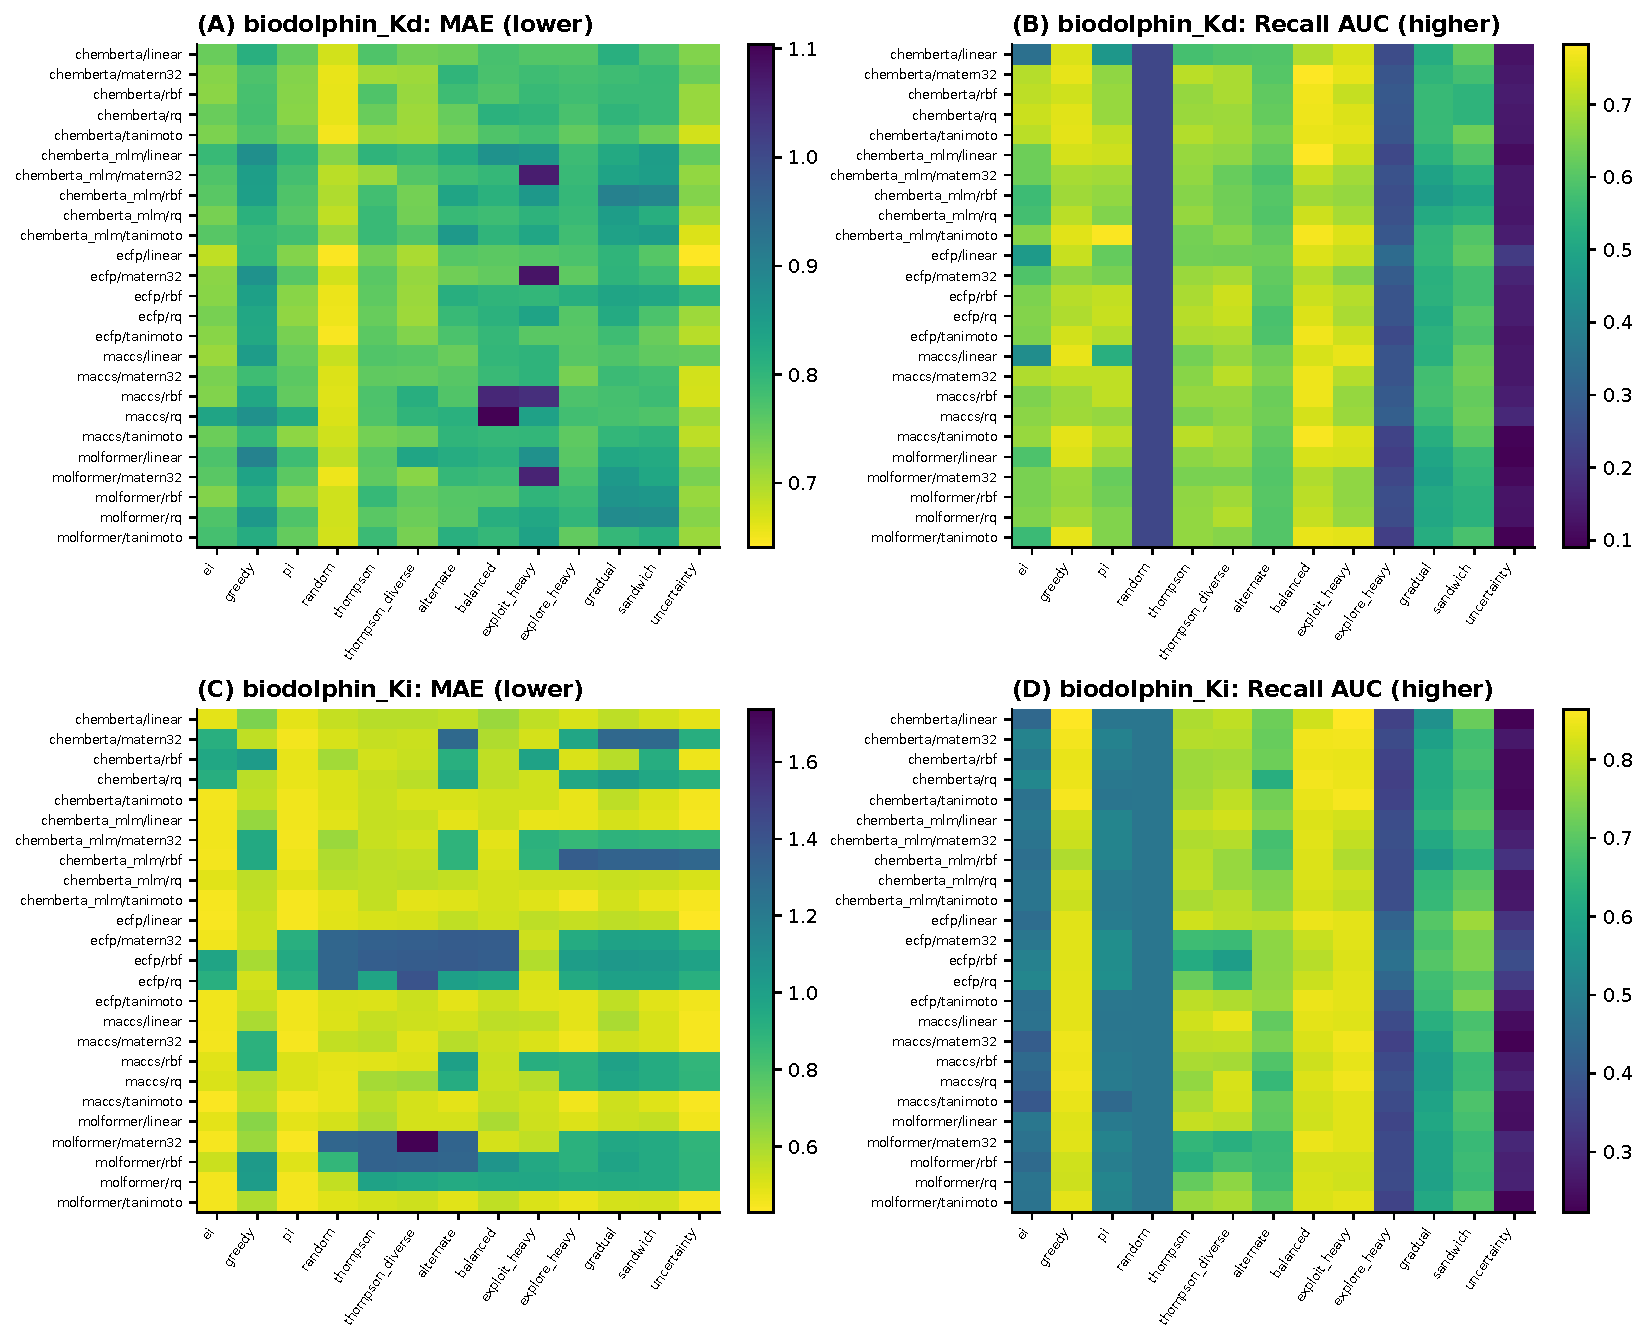
\includegraphics[width=\linewidth]{figures/fig2_grid.pdf}
\caption{Complete pooled-data representation--kernel grids in four
panels. (A,C) Final test MAE. (B,D) Label-normalized top-decile recall AUC.
Rows are representation/kernel combinations and columns are query policies.
All values are three-seed means; pooled $K_d$ and $K_i$ retain their
separate endpoint definitions.}
\label{fig:grid}
\end{figure}

\section{Results}
\subsection{Prediction and discovery select different configurations}
Table~\ref{tab:results} and Figures~\ref{fig:performance}--\ref{fig:grid}
show the central trade-off. For pooled $K_d$, ECFP--linear with uncertainty-only
selection achieves the lowest observed mean MAE, $0.641\pm0.041$, and
mean $R^2=0.665$. Its final recall is 0.338. The original grid's
random-acquisition winner remains close at $0.643\pm0.055$; this small
post-hoc difference is not evidence of statistical superiority.
The lowest-MAE Thompson configuration, ChemBERTa-MTR--Mat\'ern,
has MAE $0.705\pm0.046$ and recall
0.967. Thus high-affinity discovery does not require the lowest global
test error, and maximizing discovery need not optimize that error.

The highest recall-AUC $K_d$ configuration combines balanced UCB and
ChemBERTa-MLM--linear, yielding AUC 0.783 and final recall 0.976. This is distinct
from choosing the largest endpoint recall. On $K_i$, the lowest-MAE
configuration is ECFP--linear with uncertainty-only querying, giving
MAE $0.429\pm0.044$ and mean $R^2=0.846$, compared with the previous
lowest MAE of 0.455. Its recall AUC is 0.319 and final recall is 0.543.
ChemBERTa-MTR--linear with greedy or exploit-heavy querying ties for
highest AUC (0.864), with final recall 1.000. We retain both tied winners
in the supplementary tables; exploit-heavy has lower MAE (0.554 versus 0.689).
High endpoint recall alone can also conceal the difference
in when high-affinity pairs were acquired.

\begin{table}[t]
\centering\small
\caption{Descriptive selected pooled configurations (three seeds).
P: lowest mean MAE; D: highest mean recall AUC; T: lowest mean MAE among
Thompson models. MTR/MLM denote ChemBERTa variants; M32 is Mat\'ern-$3/2$.
Selection is post-hoc on these results, not nested validation.}
\label{tab:results}
\begin{tabular}{lllrrrr}
\toprule
Endpoint/role & Representation/kernel & Policy & MAE & $R^2$ & Recall & AUC\\
\midrule
$K_d$/P & ECFP/linear & Uncertainty & .641 & .665 & .338 & .210\\
$K_d$/D & MLM/linear & Balanced & .868 & .467 & .976 & .783\\
$K_d$/T & MTR/M32 & Thompson & .705 & .624 & .967 & .711\\
$K_i$/P & ECFP/linear & Uncertainty & .429 & .846 & .543 & .319\\
$K_i$/D & MTR/linear & Exploit-heavy & .554 & .787 & 1.000 & .864\\
$K_i$/D & MTR/linear & Greedy & .689 & .666 & 1.000 & .864\\
$K_i$/T & MACCS/RBF & Thompson & .490 & .836 & 1.000 & .784\\
\bottomrule
\end{tabular}
\end{table}

These are comparisons at the same 360-label pooled budget. An earlier
fixed-kernel benchmark used only 64 labels; its plots are retained in the
supplementary atlas but are not evidence of budget-matched improvement.
No claim of superiority over external state-of-the-art methods follows
from the present grid.

\subsection{Tiny target panels do not establish reliable prediction}
Even the lowest-MAE selected configurations have negative mean $R^2$
on every small panel: $-0.217$ and $-0.265$ on TRAAK-a and TRAAK-b,
and $-2.601$ and $-1.138$ on TTR-A and TTR-B. These are the
lowest-MAE selections, not selections by maximum $R^2$. Their test sets contain
only two or three pairs. A small absolute MAE on a narrow affinity range
does not establish useful ranking or extrapolation. Some final-model
lipid attributions are nearly zero, consistent with weak discrimination
on the explained examples. Protein attribution is zero on a fixed-protein
panel by construction, not evidence that the protein is biologically
irrelevant. Small-panel high recall is also easy to obtain when much of
the acquisition pool has been measured.

\begin{figure}[t]
\centering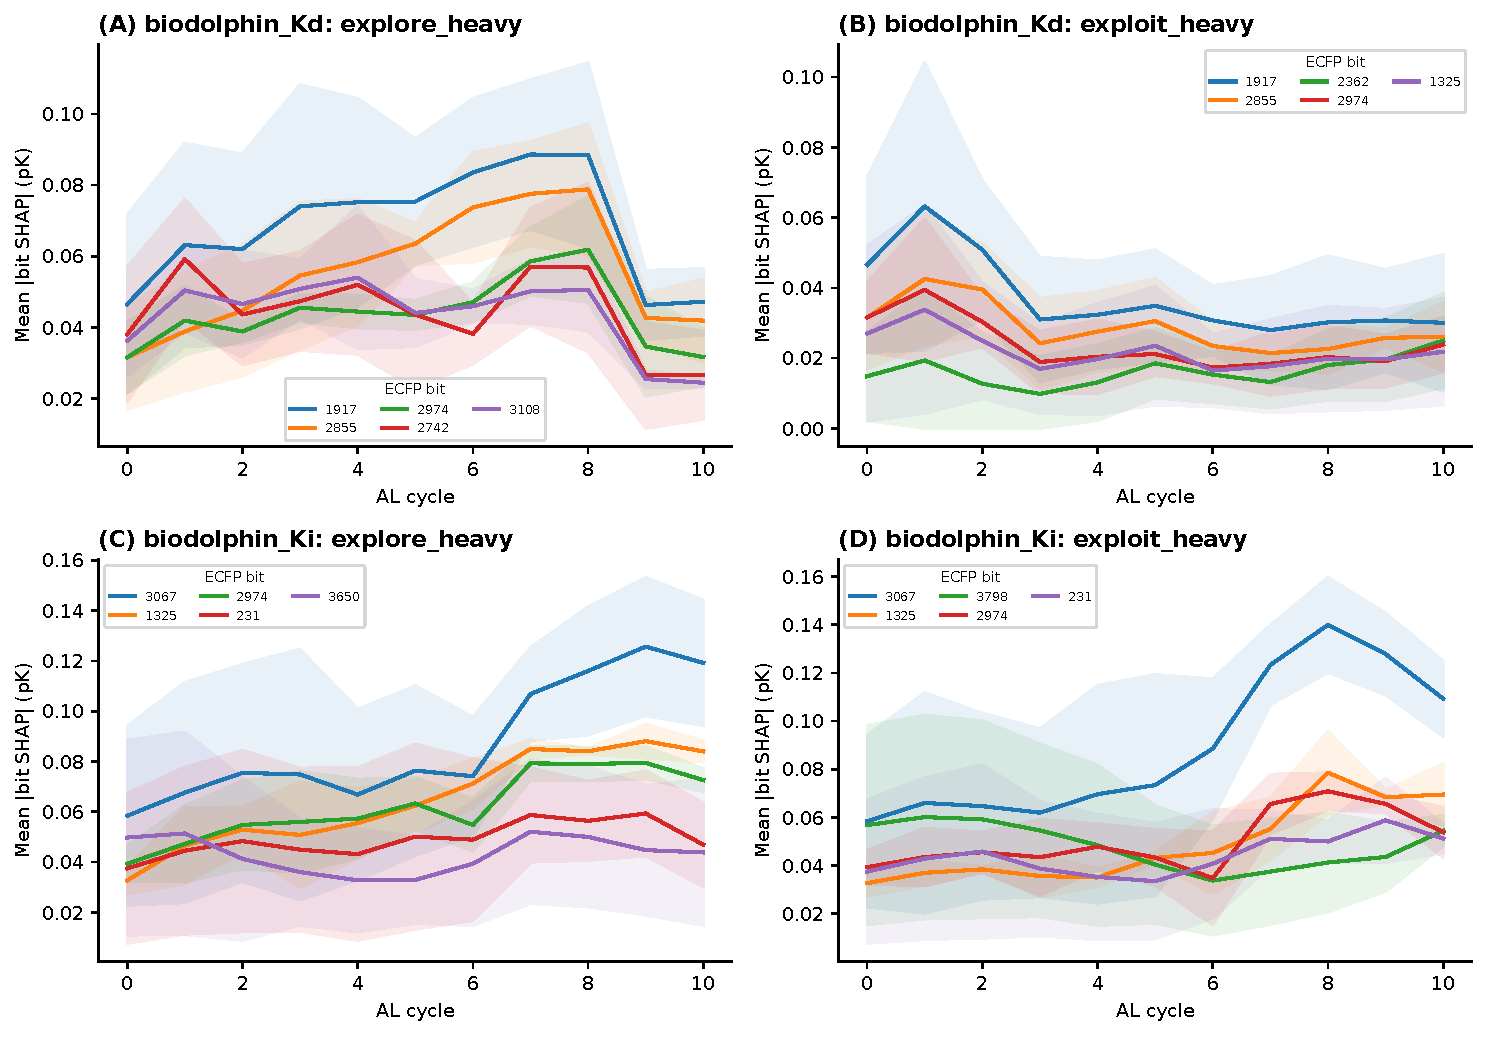
\includegraphics[width=\linewidth]{figures/fig3_temporal.pdf}
\caption{Four temporal explanation panels for matched ECFP--linear
campaigns. The five bits with largest final importance averaged across
seeds are shown in each panel. Lines are seed means; bands are seed
standard deviations. Explore-heavy uses $E^7X^3$ and exploit-heavy
uses $X^7E^3$. Importance reflects model, query population and background
together; it need not increase monotonically with measurement count.}
\label{fig:temporal}
\end{figure}

\subsection{Frozen transformers do not uniformly improve affinity learning}
Figure~\ref{fig:representations} fixes Mat\'ern-$3/2$ and Thompson sampling
to compare all five encodings without changing policy or kernel. On $K_d$,
mean MAEs are 0.759 (ECFP), 0.753 (MACCS), 0.705 (MTR), 0.711 (MLM),
and 0.753 (MoLFormer). On $K_i$ they are 1.329, 0.566, 0.542, 0.540,
and 1.328, respectively. Thus the additional encoders do not monotonically
improve prediction; the small MLM--MTR difference on $K_i$ is descriptive.
Representation rankings depend on kernel and policy: the overall predictive
winners on both pooled endpoints remain ECFP--linear with uncertainty-only
acquisition. Frozen molecular pretraining, assay heterogeneity and coarse
protein features are plausible contributors, not experimentally isolated causes.

\begin{figure}[t]
\centering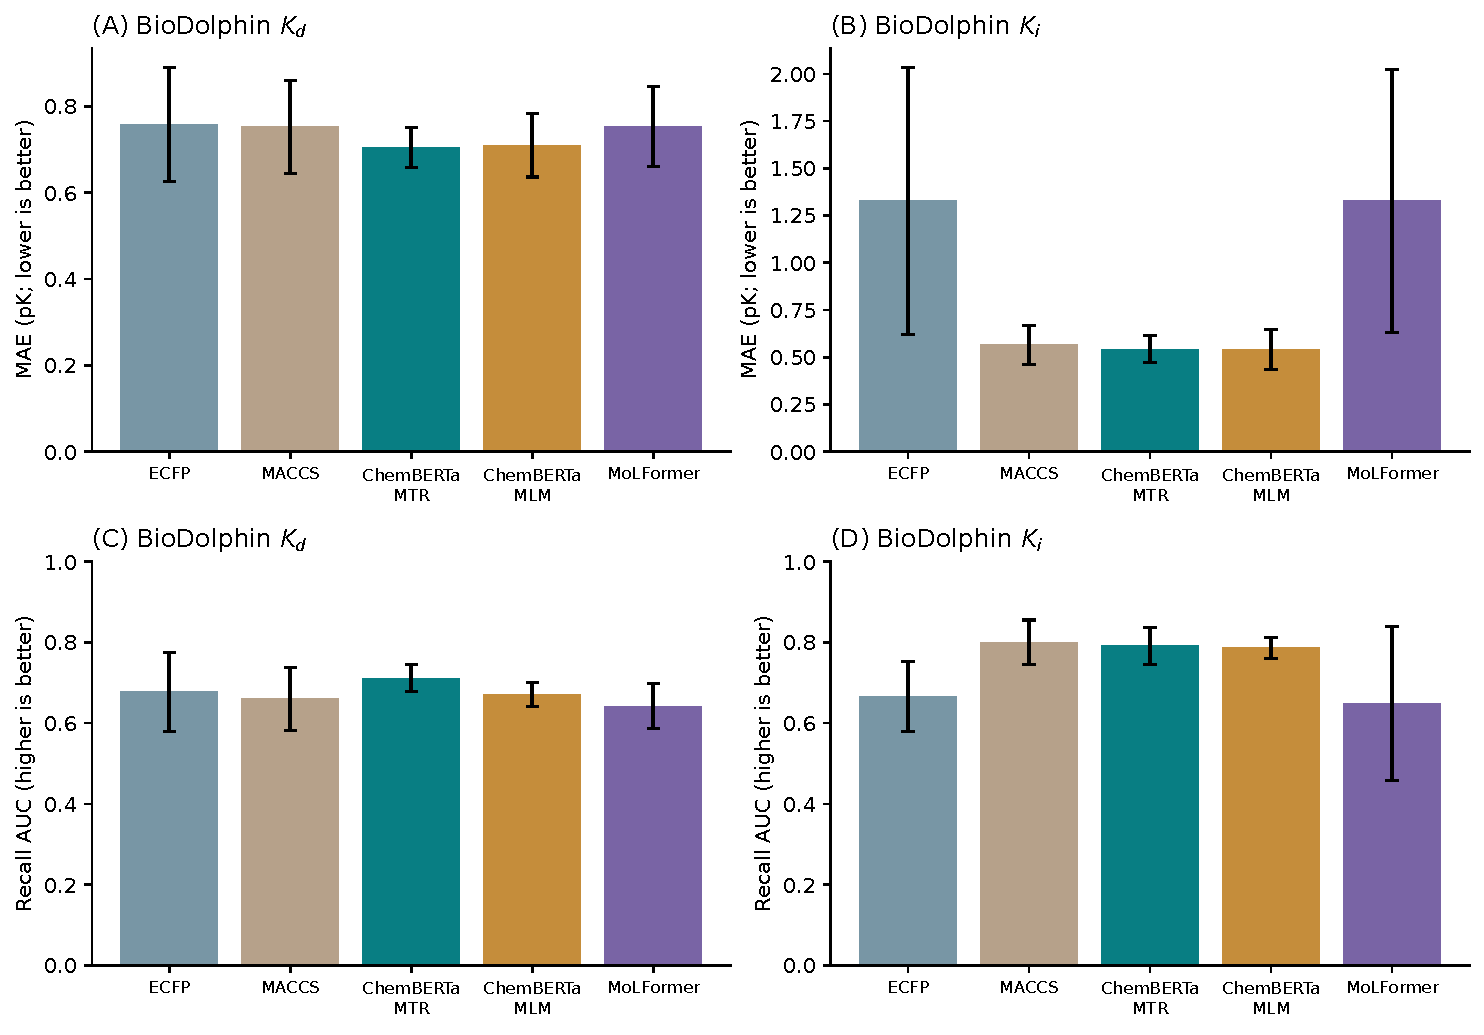
\includegraphics[width=\linewidth]{figures/fig6_representations.pdf}
\caption{Matched representation comparison in four panels. All encoders use
Mat\'ern-$3/2$, joint Thompson sampling, identical splits and the same label
budget. (A,B) Final held-out MAE. (C,D) Label-normalized discovery AUC.
Bars and whiskers are three-seed means and sample SD, not confidence intervals.
MTR and MLM denote the two frozen ChemBERTa checkpoints.}
\label{fig:representations}
\end{figure}

\subsection{Attribution fidelity and chemical interpretation}
The grouped analysis explains 234 test-pair/model instances across 54
models. Rebuilt posterior means match saved predictions to at most
$2.72\times10^{-13}$ pK; additive reconstruction error is at most
$1.30\times10^{-13}$ pK. The largest model-level mean absolute
difference between the two permutation-SHAP repetitions is 0.0262 pK.
This checks sampling sensitivity at the chosen background, not robustness
to alternative backgrounds or to a different model.

For selected Thompson models, mean absolute two-player contributions
averaged across seeds are 0.802 pK for lipid and 0.835 pK for protein
on $K_d$, and 1.012 versus 0.899 pK on $K_i$. They are not percentages
of predictive accuracy and should not be compared as causal effect sizes.
The detailed temporal analysis yields 14,754 pair/model explanations.
Its maximum additive reconstruction error is $9.86\times10^{-14}$ pK;
the 36 independent KernelExplainer checks disagree by at most
$9.23\times10^{-11}$ pK. Exact agreement is expected for the affine
game and is not evidence of a correct biochemical model.

Temporal rankings vary (Figure~\ref{fig:temporal}). Final top-ten
Jaccard overlap between explore-heavy and exploit-heavy averages 0.545
on both pooled endpoints. Active-bit rank correlations average 0.642
for $K_d$ and 0.597 for $K_i$. These moderate agreements do not support
protocol-independent motif rankings. The supplementary highlighted
fragments provide concrete annotations of bit environments. Their
affinity-prioritized selection deliberately favors potent examples,
so the resulting visual association is not an independent SAR test.
Figure~\ref{fig:fragments} gives four representative chemical panels;
different important environments may be drawn from the same potent molecule.

\begin{figure}[t]
\centering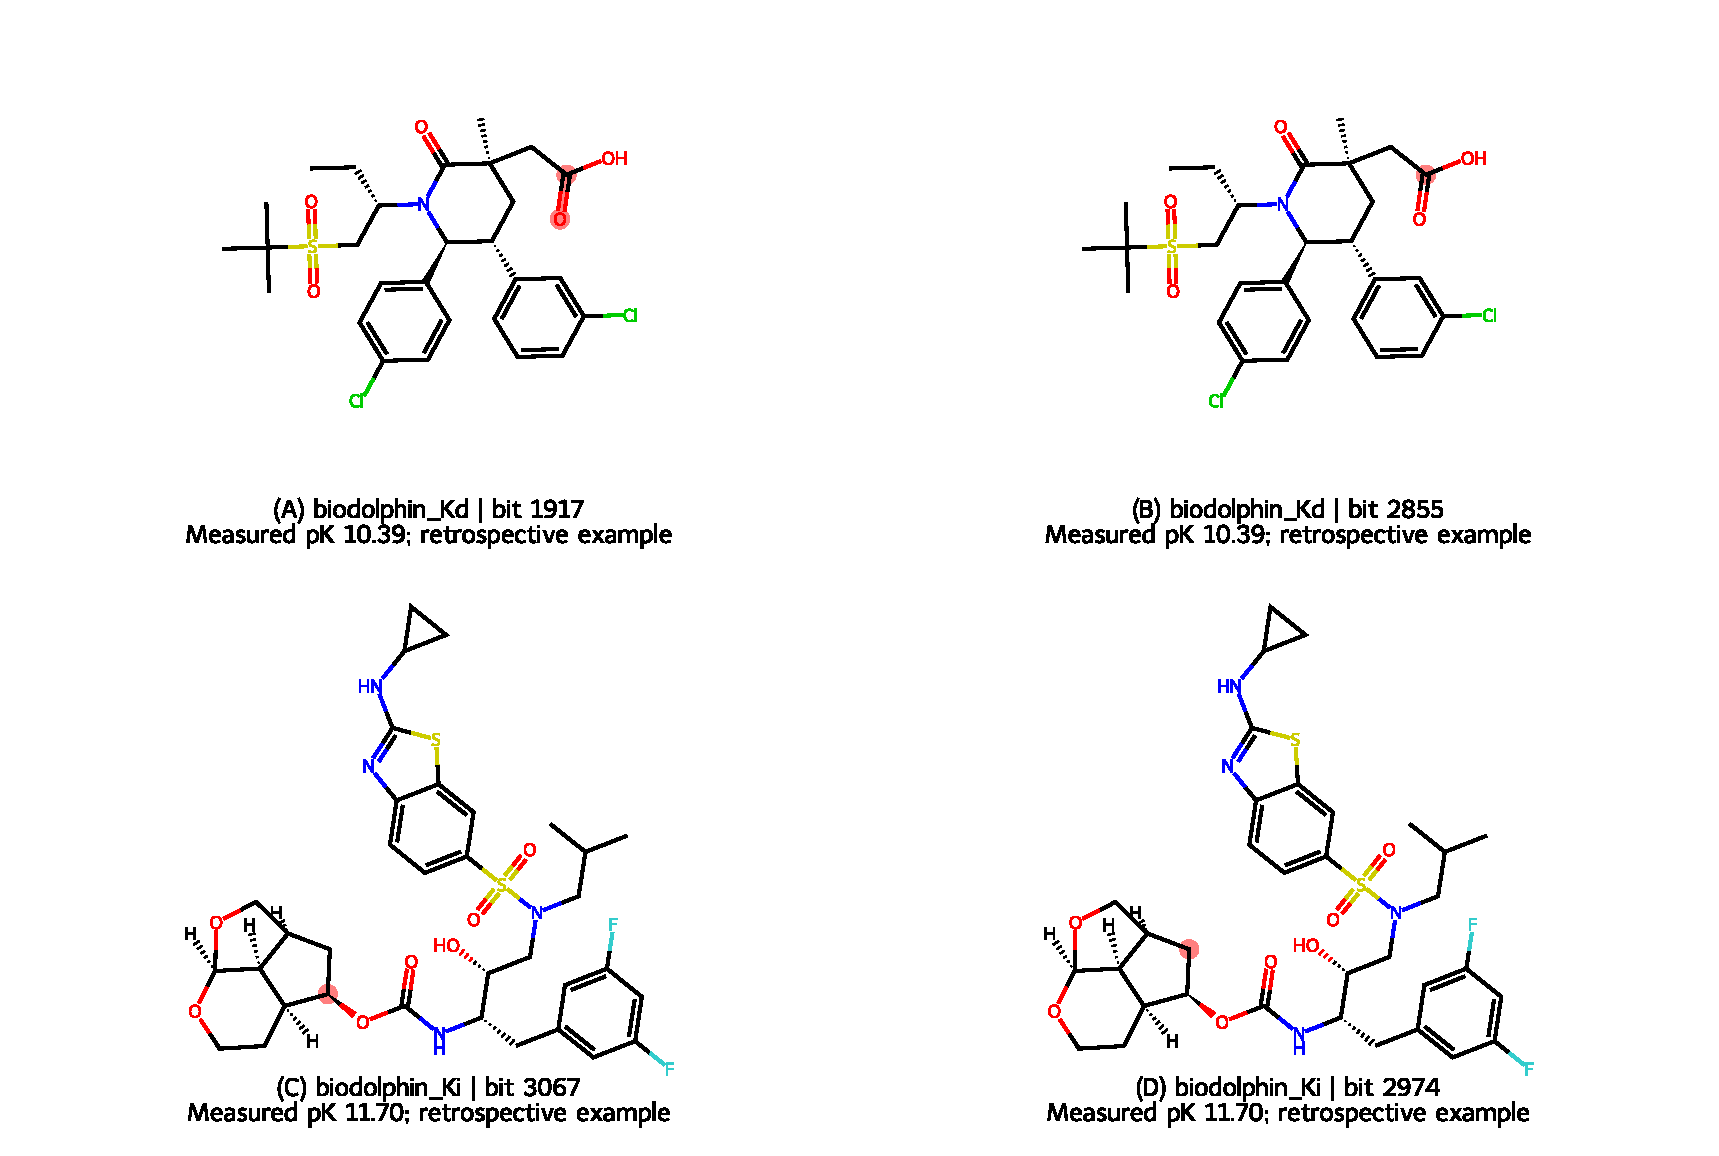
\includegraphics[width=\linewidth]{figures/fig5_fragments.pdf}
\caption{Four affinity-prioritized molecular examples from seed-7
ECFP--linear explore-heavy campaigns: two highest combined-score bits for
pooled $K_d$ (A,B) and $K_i$ (C,D). Highlighted atoms mark one recorded
ECFP environment, not a binding site. Whole molecules are shown to preserve
chemical context. Examples use retrospective measured labels and may repeat
the same molecule for different bits; they are not four independent hits or
evidence of causal interactions. Full collision records appear in the atlas
and source outputs.}
\label{fig:fragments}
\end{figure}

\begin{figure}[t]
\centering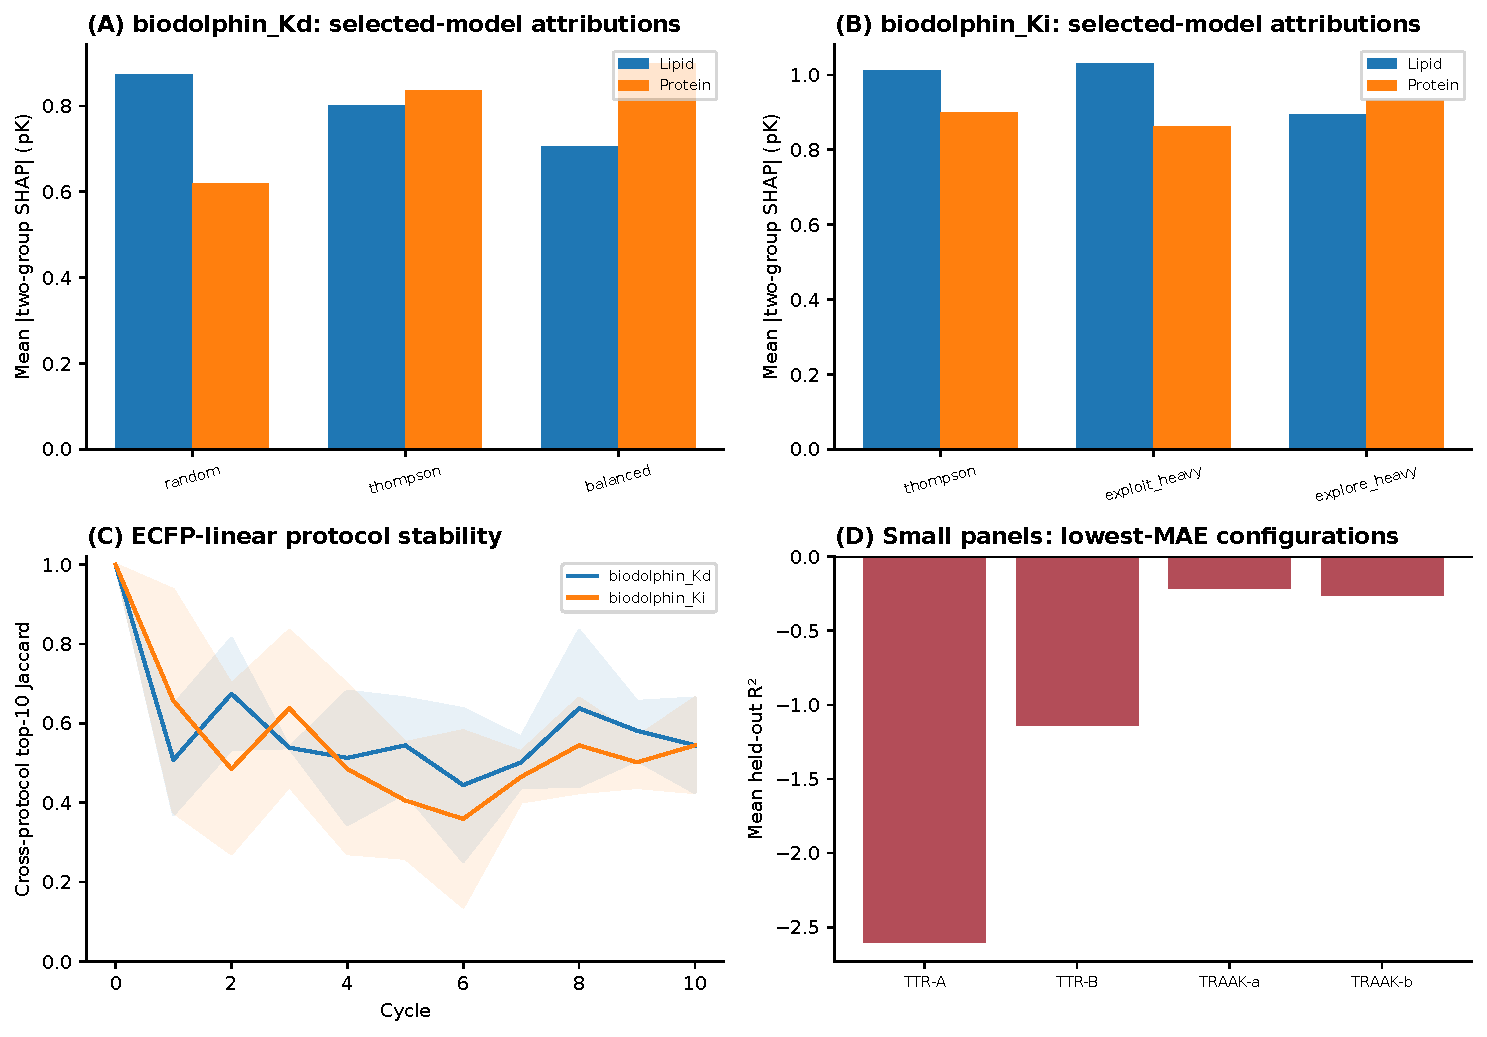
\includegraphics[width=\linewidth]{figures/fig4_explanations.pdf}
\caption{Four-panel interpretability and reliability summary. (A,B)
Mean absolute two-player SHAP values for the selected final-model
configurations selected from the original grid, averaged across seeds and their explained subsets;
representations/kernels differ between selections. (C) Matched
ECFP--linear protocol overlap, with seed SD bands. (D) Negative mean
$R^2$ persists on all small panels even for lowest-MAE configurations.}
\label{fig:explanations}
\end{figure}

\subsection{Execution and reproducibility checks}
All 5,850 expected runs are present. Split separation, matched
initialization, phase schedules and label budgets pass the recorded
audit. Of 48,750 fits, 48,724 meet the optimizer convergence criterion;
26 do not. These
are explicitly logged, not silently described as converged. On the
54 selected explanation campaigns, reconstructing saved posteriors and
replaying original random-number streams reproduces selected indices
in all 396 nonempty acquisition rounds. Final-prediction SHAP is distinct
from this acquisition replay: it does not explain a particular Thompson
function draw. Independent tests cover covariance calculations, analytic
gradients, saved-prediction agreement and masked-feature predictions.
Additional checks exercise all 325 representation--kernel--policy combinations
on measured TRAAK data, transformer determinism and padding invariance, and
actual browser upload campaigns. These are computational checks, not evidence
of model generalization.

\section{Interactive Dashboard and Deployment Scope}
The LipidLab portal (Figure~\ref{fig:dashboard}) exposes all 5,850 benchmark
runs through linked dataset, representation, kernel, policy and seed controls.
Four-panel curves show held-out MAE, discovery recall, RMSE and interval
coverage. A matched representation table reports seed means and SD; audit
downloads expose numerical results. Separate views retain 90 explanation
reports (54 grouped and 36 temporal), explicitly marking missing SHAP rather
than equating a benchmark result with an explanation.

The local Flask service accepts measured CSV pairs, validates sequences,
SMILES, affinity units and budgets, and runs retrospective AL using the same
supported encoders, kernels and policies. Test rows remain excluded from
acquisition; progress, cancellation and result downloads are available. New
uploads do not automatically generate SHAP or prospective experimental labels.

A read-only static export is prepared for Vercel hosting. It excludes user
uploads, pretrained weights and the Python execution environment. A public
deployment has not been verified and no public URL is claimed in this draft.
The screenshots show the functioning local application. The current in-memory
job queue and local output files are not a durable hosted-job architecture;
online AL would require a separately provisioned service with persistent job
state, storage, authentication and resource limits. Merely hosting the static
page does not make its upload runner executable. An anonymous hosting URL
should be added only after deployment and review of data redistribution and
conference anonymity requirements.

\begin{figure}[t]
\centering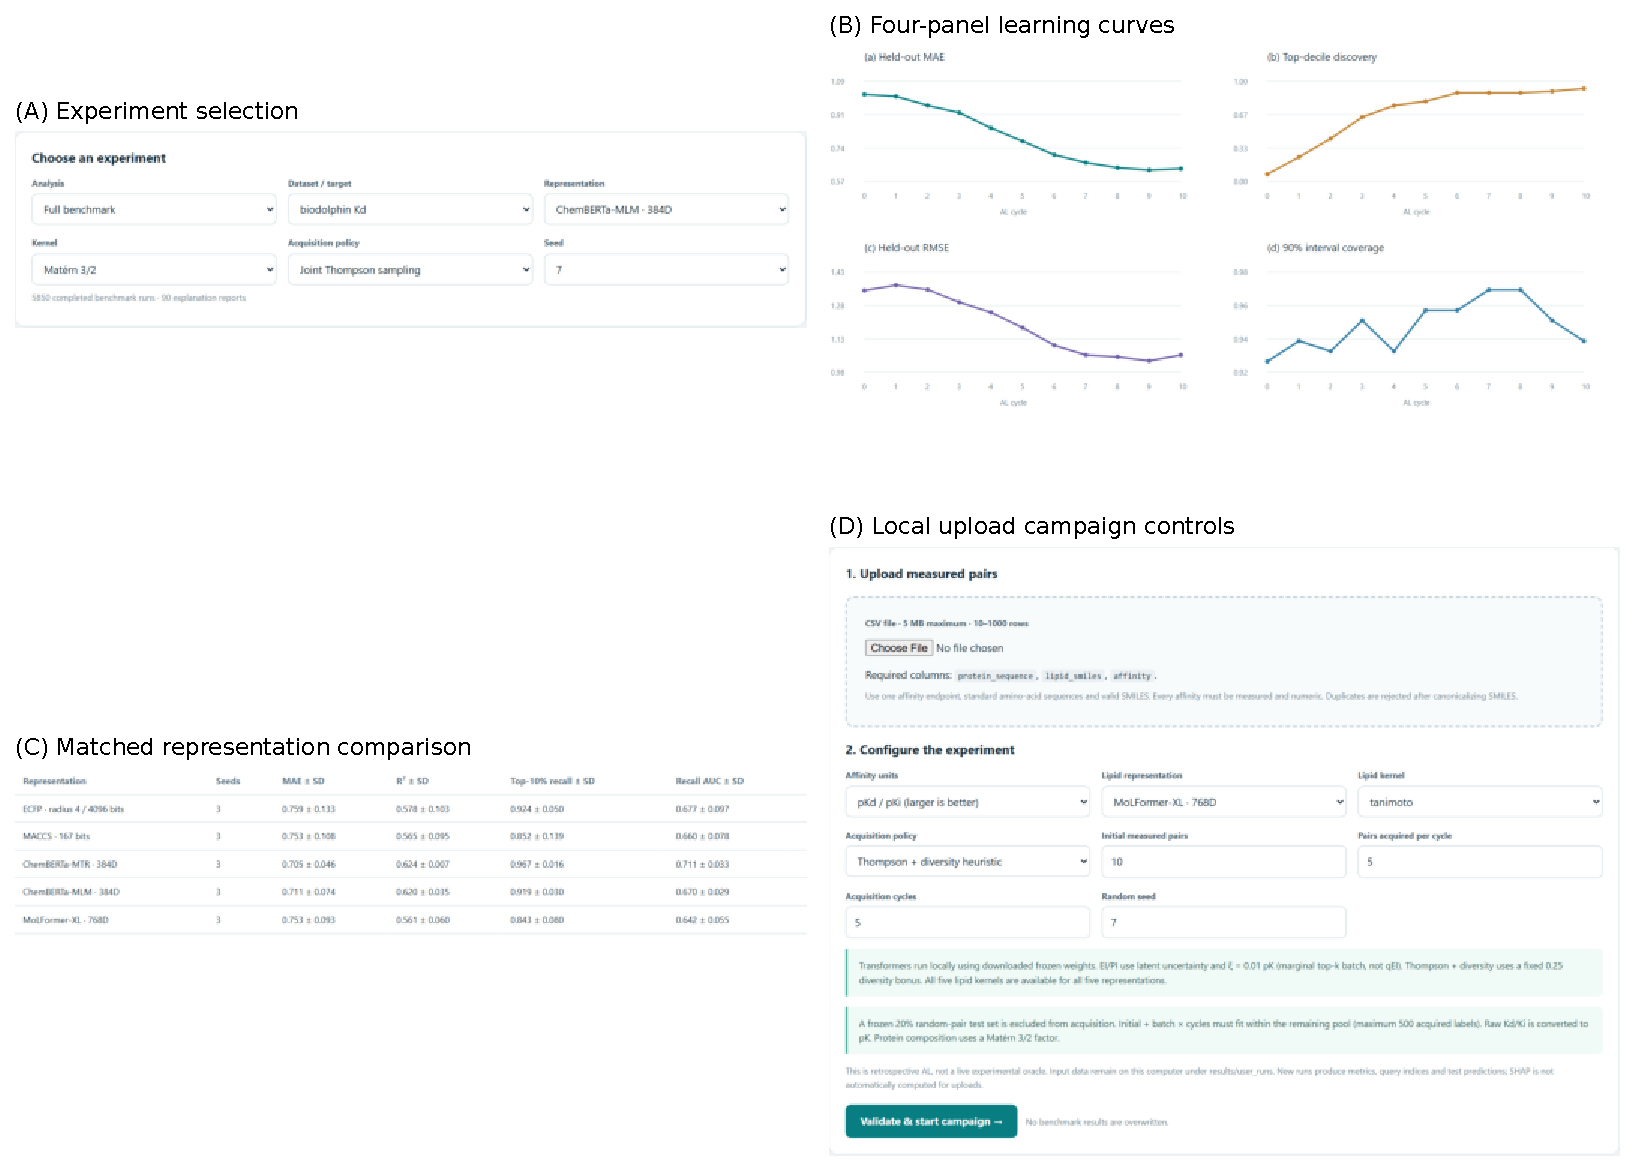
\includegraphics[width=\linewidth]{figures/fig7_dashboard.pdf}
\caption{Four screenshots of the actual local dashboard: (A) linked experiment
selection, (B) learning-curve panels, (C) matched representation comparison,
and (D) upload/campaign controls. The displayed results come from completed
published-data experiments; the controls do not imply a public hosted AL
service. The screenshot source and hashes accompany the source package.}
\label{fig:dashboard}
\end{figure}

\section{Limitations and Discussion}
\paragraph{Generalization and selection.}
Random-pair splits permit homologous proteins and related chemical
structures across train and test. They do not measure cold-target,
cold-family or scaffold generalization. Nested selection, grouped splits
and more seeds are needed before selecting a deployment model. The
configuration grid is a controlled comparison, not 1,950 independent
replications. TTR panels overlap the pooled data. Uncertainty calibration
is recorded but not sufficient to establish out-of-distribution reliability.

\paragraph{Assay and dataset scope.}
Heterogeneous experimental conditions and consensus labels can introduce
unmodeled variation. BioDolphin's structural-resource scale must not be
equated to the number of independent measured affinities used here.
The broad lipid definition also prevents interpreting every result as
membrane-phospholipid recognition. Dedicated larger, homogeneous
target-specific affinity panels would strengthen the benchmark.

\paragraph{Explanation scope.}
Marginal feature replacement may create invalid fingerprint combinations.
Protein-conditioned pooled explanations aggregate over different targets,
so a recurring bit need not be a universal binding determinant. A
representative fragment cannot resolve every collision. Numerical
additivity neither establishes causal necessity nor verifies a binding
site. No contact maps, docking validation, residue importance or prospective
mutagenesis results are claimed. Background-sensitivity and fixed-population
temporal controls would help separate model evolution from population drift.

\paragraph{Methodological scope.}
The most extensive per-bit analysis uses only the linear lipid kernel.
Extending ungrouped explanations to non-linear kernels requires additional
computation and convergence checks rather than reuse of the affine shortcut.
The protein product kernel and optimizer differ from the reference study.
Our evidence supports a transparent adaptation and objective trade-off,
not a new theory of active learning or a universally optimal policy.

\section{Conclusion}
In this retrospective protein--lipid study, acquisition enrichment and
global predictive accuracy are distinguishable outcomes. Thompson sampling
and scheduled UCB can prioritize high-affinity pairs while uncertainty-only
querying gives the lowest descriptive prediction error in the expanded grid.
Adding frozen transformers does not guarantee improvement. Small target panels
remain insufficient for reliable predictive claims. Temporal ECFP
attributions and fragment annotations make model behavior inspectable,
but their fidelity must not be confused with biological validity. Stronger
evidence requires target-aware evaluation, homogeneous measurements,
robust explanation controls and prospective testing.

\section*{Reproducibility and Supplementary Material}
The accompanying source package contains this manuscript, seven four-panel
figures and the complete figure atlas. The atlas includes every one of
223 pre-existing result figures in 45 composite figures with four or five
source panels each, including legacy-budget plots, full-grid heatmaps,
54-model grouped explanations, and temporal/chemical plots for all 36
campaigns. A CSV manifest maps every panel to its source and SHA-256 hash.
Full expanded-grid summaries (1,950 configurations), per-seed outcomes
(5,850 campaigns), tied-winner tables and execution audit accompany the paper.
The new representation and dashboard composites are separate from the legacy
223-source atlas. Original checkpoints and measurements are not modified by manuscript
generation. Configuration and data hashes identify the computations.
The separate atlas is supplementary material, not part of the main-paper
page budget, and does not substitute for the evidence summarized above.

\begin{thebibliography}{9}
\bibitem[DeepChem(n.d.)]{chemberta}
DeepChem. ChemBERTa-77M pretrained molecular checkpoints, MTR and MLM.
\url{https://huggingface.co/DeepChem/ChemBERTa-77M-MTR};
\url{https://huggingface.co/DeepChem/ChemBERTa-77M-MLM}.
Pinned revisions are recorded in the feature manifest.
\bibitem[Ross et~al.(2022)]{ross2022}
Jerret Ross, Brian Belgodere, Vijil Chenthamarakshan, Inkit Padhi,
Youssef Mroueh, and Payel Das.
Large-scale chemical language representations capture molecular structure and properties.
\emph{Nature Machine Intelligence}, 4:1256--1264, 2022.
\doi{10.1038/s42256-022-00580-7}.
\bibitem[Rasmussen and Williams(2006)]{rasmussen2006}
Carl Edward Rasmussen and Christopher K. I. Williams.
\emph{Gaussian Processes for Machine Learning}. MIT Press, 2006.
\url{https://gaussianprocess.org/gpml/}.
\bibitem[Russo et~al.(2018)]{russo2018}
Daniel Russo, Benjamin Van Roy, Abbas Kazerouni, Ian Osband, and Zheng Wen.
A tutorial on Thompson sampling.
\emph{Foundations and Trends in Machine Learning}, 11(1):1--96, 2018.
\doi{10.1561/2200000070}.
\bibitem[Rogers and Hahn(2010)]{rogers2010}
David Rogers and Mathew Hahn.
Extended-connectivity fingerprints.
\emph{Journal of Chemical Information and Modeling}, 50(5):742--754, 2010.
\doi{10.1021/ci100050t}.
\bibitem[Yang et~al.(2024)Yang, Ping, and Luo]{yang2024}
Li-Yen Yang, Kaike Ping, and Yunan Luo.
BioDolphin as a comprehensive database of lipid--protein binding interactions.
\emph{Communications Chemistry}, 7:288, 2024.
\doi{10.1038/s42004-024-01384-z}.
\bibitem[Schrecke et~al.(2021)]{schrecke2021}
Samantha Schrecke, Yun Zhu, Jacob W. McCabe, Mariah Bartz, Charles Packianathan,
Minglei Zhao, Ming Zhou, David Russell, and Arthur Laganowsky.
Selective regulation of human TRAAK channels by biologically active phospholipids.
\emph{Nature Chemical Biology}, 17:89--95, 2021.
\doi{10.1038/s41589-020-00659-5}.
\bibitem[Srivastava et~al.(2026)]{srivastava2026}
Satya Pratik Srivastava, Rohan Gorantla, Sharath Krishna Chundru,
Claire J. R. Winkelman, Antonia S. J. S. Mey, and Rajeev Kumar Singh.
Explainable active learning framework for ligand binding affinity prediction.
\emph{Digital Discovery}, 5:769--779, 2026.
\doi{10.1039/D5DD00436E}.
\bibitem[Lundberg and Lee(2017)]{lundberg2017}
Scott M. Lundberg and Su-In Lee.
A unified approach to interpreting model predictions.
\emph{Advances in Neural Information Processing Systems}, 30, 2017.
\url{https://arxiv.org/abs/1705.07874}.
\end{thebibliography}
\end{document}
